\chapter{I Had to Beg, Borrow, and Steal: Capital, Control, and the Arithmetic of Scale}

This chapter is based on a School of Hard Knocks interview with Louis, a Houston entrepreneur whose labor-force management company is described in the transcript as doing about \$300 million in annual revenue. The chapter is curated by LazyingArt LLC through Video2Book. There are no validated blackboard images for this lecture, so the mathematical structure below is reconstructed from the spoken claims: rough ratios, working-capital timing, invoice factoring, retained earnings, equity control, and results-based negotiation.

\section{The First Number: Delegation as a Multiplier}

The interview begins with visible proof: a Ferrari, a Houston street interview, a \$300 million entrepreneur, and a private car collection. But the first real mechanism is not the car. It is delegation. When asked how important it was to master delegation, Louis answers by comparing the company as it operates now with the company as it would exist if he were still doing the work himself.

Let
\[
R_{\mathrm{delegated}} \approx \$300\text{M/year},
\qquad
R_{\mathrm{solo}} \approx \$3\text{M/year}.
\]
The implied scale factor is
\begin{equation}
L_{\mathrm{delegation}}
   \approx
   \frac{R_{\mathrm{delegated}}}{R_{\mathrm{solo}}}
   \approx
   \frac{300}{3}
   =
   100.
\end{equation}

This is not a proof that delegation alone caused a hundredfold increase. It is an interview claim used as a measuring device. It tells us what the speaker wants us to see first: the entrepreneur is not merely a high-performing individual. The entrepreneur has built an organization that can act beyond one person's hands.

\subsection{Question \& Answer}

\paragraph{Question.} What did delegation multiply?

\paragraph{Answer.} It multiplied operating capacity. Louis says that if he were still doing everything himself, the business might do about \$3 million. With a delegated company, he describes about \$300 million in annual revenue. The point is not that delegation is a magic constant; the point is that the business crossed from personal labor into organized labor, systems, and management.

\section{What Was Actually Being Sold?}

The next beat is essential. The interviewer asks what type of business Louis runs, and Louis says that FX is a labor-force management company. He says that companies across the United States outsource their entire labor force to his company.

That statement should be read carefully. The product is not simply ``hours of labor'' in the abstract. The transcript presents a more complete operating object:
\begin{itemize}
\item a customer company with a labor-force problem,
\item a provider that can manage that labor force,
\item contracts large enough to require financing,
\item operating procedures and training that make performance repeatable,
\item relationships strong enough for clients to turn over more business.
\end{itemize}

So the business object is a managed labor system. A customer is not merely buying workers; it is buying a more reliable operating arrangement.

\begin{definition}
A \emph{managed labor-force contract}, in the sense used in this chapter, is a commercial arrangement in which a customer transfers responsibility for a substantial labor function to an outside operator. The operator must then finance, staff, manage, and improve the work before all cash from the customer has necessarily arrived.
\end{definition}

This definition matters because the financing problem later in the interview only makes sense if the contracts are large and cash-hungry. A small service sale might be funded by the owner's pocket. A nationwide labor contract can create a working-capital gap before it creates wealth.

\section{Mindset, Risk, and the Spending Trap}

Before Louis gives the working-capital arithmetic, the conversation passes through mindset and spending. This is not filler. It is part of the causal chain.

Louis says mindset matters more than skill set because skills can be taught but passion and drive cannot simply be handed over. He also says entrepreneurship is not for everyone. The risk, the stress, and the mental toll can make it the wrong game for many people.

Then the interview turns to why people stay broke. Louis points to spending, leverage, and buying things with no return on investment. The claim about ``one in four millionaires'' living paycheck to paycheck should be preserved as an interview claim, not treated here as an independently verified statistic. But the mechanism is clear enough:

\begin{equation}
\text{financial fragility}
\quad\hbox{increases when}\quad
\text{consumption debt} > \text{productive investment}.
\end{equation}

That personal-finance point immediately becomes a business-finance point. Louis says that when the company was making money, every dollar had to stay in the company to reduce the next week's debt liabilities. The owner could not behave like a consumer if the business needed capital to survive.

A compact way to write the rule is
\begin{equation}
D_{t+1} \approx D_t - RE_t,
\end{equation}
where \(D_t\) is the borrowing need or debt liability at time \(t\), and \(RE_t\) is retained earnings left inside the company. The equation is deliberately simple. It is not a full accounting model. It captures the spoken discipline: leave cash in the business, borrow less next time, and let the balance sheet become stronger.

\section{Seed Money, Control, and the Cost of an Idea}

The interviewer then asks the capital question directly. Many people need money to start or grow a business. Louis had said earlier that he had to beg, borrow, and steal to get started. Now he explains the tradeoff.

If a founder comes to an investor with only an idea, the investor is taking the financial risk. The founder may risk time and effort, but if the deal fails, the investor's money is gone. Therefore, Louis says, the investor will want control over how the money is spent. In equity terms, that often means majority ownership.

The transcript gives two useful ownership markers:
\begin{align}
s_{\mathrm{investor}} &\geq 51\%,\\
s_{\mathrm{investor}} &\approx 70\%, \qquad
s_{\mathrm{founder}} \approx 30\%.
\end{align}

Again, these are not universal venture-capital laws. They are Louis's spoken description of how seed money can work when the investor is carrying the financial downside.

\subsection{Question \& Answer}

\paragraph{Question.} Why does outside capital cost control?

\paragraph{Answer.} Because money carries downside. If the investor supplies the capital before there is proof of execution, the investor bears the financial loss if the business fails. Louis's argument is that the investor then wants control over spending, and control appears as majority equity or a split like 70/30. The founder who arrives with revenue and proof is not asking someone to fund a raw idea; the founder is asking someone to fund scale.

\begin{figure}
\centering
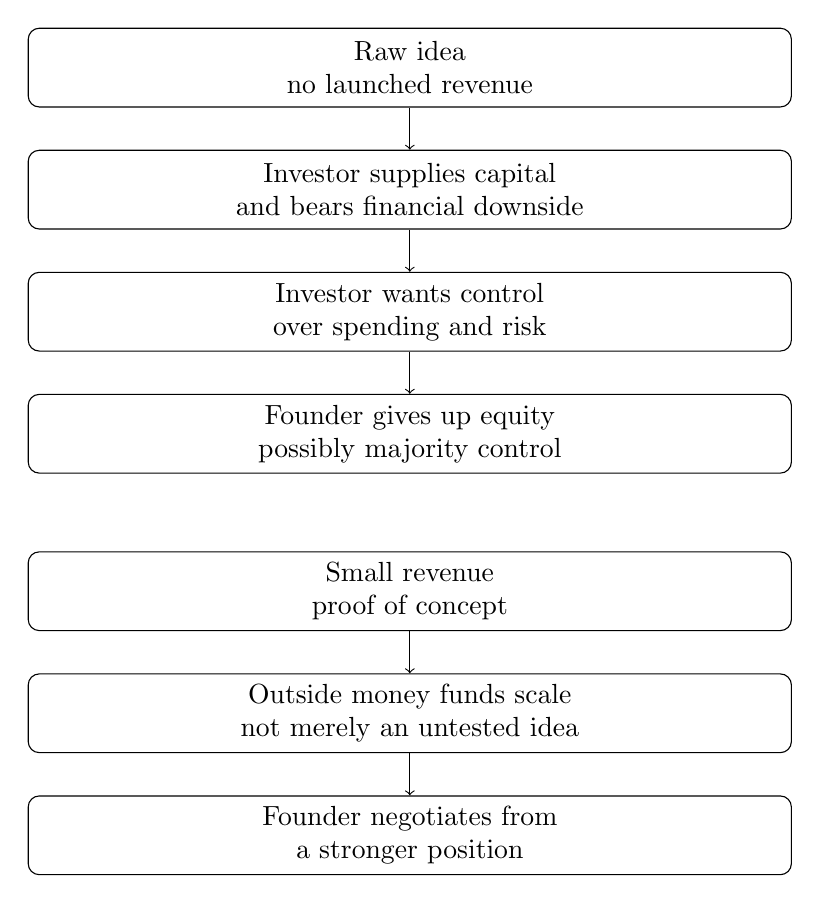
\begin{tikzpicture}[
  node/.style={draw, rounded corners, align=center, text width=0.78\linewidth, minimum height=1.0cm},
  smallnode/.style={draw, rounded corners, align=center, text width=0.62\linewidth, minimum height=0.9cm},
  yscale=1.0
]
\node[node] (idea) at (0,0) {Raw idea\\no launched revenue};
\node[node] (investor) at (0,-1.55) {Investor supplies capital\\and bears financial downside};
\node[node] (control) at (0,-3.10) {Investor wants control\\over spending and risk};
\node[node] (dilution) at (0,-4.65) {Founder gives up equity\\possibly majority control};

\node[node] (proof) at (0,-6.65) {Small revenue\\proof of concept};
\node[node] (scale) at (0,-8.20) {Outside money funds scale\\not merely an untested idea};
\node[node] (leverage) at (0,-9.75) {Founder negotiates from\\a stronger position};

\draw[->] (idea) -- (investor);
\draw[->] (investor) -- (control);
\draw[->] (control) -- (dilution);
\draw[->] (proof) -- (scale);
\draw[->] (scale) -- (leverage);
\end{tikzpicture}
\caption{Transcript-derived capital path: raw ideas tend to invite investor control, while proof of concept improves the founder's negotiating position.}
\end{figure}

\section{Invoice Factoring and the Working-Capital Gap}

Now the lecture becomes most quantitative. Louis describes the first major deal as about \$9 million a year, annualized. The customer needed 30-day pay terms. But the company still had to pay expenses while waiting for customer cash. He says that with 30-day terms plus the fifth week of expenses going out, the business was looking at about five weeks to cash-flow, requiring about \$1 million.

Let
\[
R_1 \approx \$9\text{M/year},
\qquad
T_{\mathrm{pay}} = 30\text{ days},
\qquad
N_{\mathrm{weeks}} \approx 5.
\]
A cautious working-capital approximation is
\begin{equation}
B_{\mathrm{needed}} \approx E_{\mathrm{week}}\,N_{\mathrm{weeks}},
\end{equation}
where \(E_{\mathrm{week}}\) is the weekly cash outflow that must be funded before payment arrives. Louis gives the resulting estimate directly:
\begin{equation}
B_{\mathrm{needed}} \approx \$1\text{M}.
\end{equation}

\subsection{A Worked Cash-Flow Reconstruction}

We should not reverse-engineer a precise payroll model, because payroll margins and expense timing are not given. But we can reconstruct the logic of the estimate.

\begin{enumerate}
\item A customer contract produces about \$9 million per year in annualized revenue.
\item The customer does not pay immediately; the stated term is 30 days.
\item Expenses continue while payment is pending.
\item Louis adds the fifth week of expenses going out before the first payment arrives.
\item The business therefore needs a cash bridge for roughly five weeks.
\item Louis estimates that bridge at about \$1 million.
\end{enumerate}

The annualized revenue number gives a rough weekly revenue scale:
\begin{equation}
\frac{\$9\text{M}}{52}
\approx
\$173{,}000\text{ per week}.
\end{equation}
Five weeks of revenue would be about
\begin{equation}
5 \times \$173{,}000 \approx \$865{,}000,
\end{equation}
which is close enough to Louis's rough ``about a million'' estimate to show the order of magnitude. This is only a scale check. The actual cash need depends on payroll, gross margin, taxes, timing, and other expenses.

Louis then turns to invoice factoring, also called accounts receivable factoring. Each week the company presents invoices. The factoring company buys or advances against those invoices. Louis says the advance was around 90 percent of invoice value and that the all-in cost was about 21 percent.

If \(I\) is the invoice face value, the approximate cash advance is
\begin{equation}
A_{\mathrm{cash}} \approx 0.90 I.
\end{equation}
The cost is described as
\begin{equation}
i_{\mathrm{factoring}} \approx 21\%.
\end{equation}

\begin{figure}
\centering
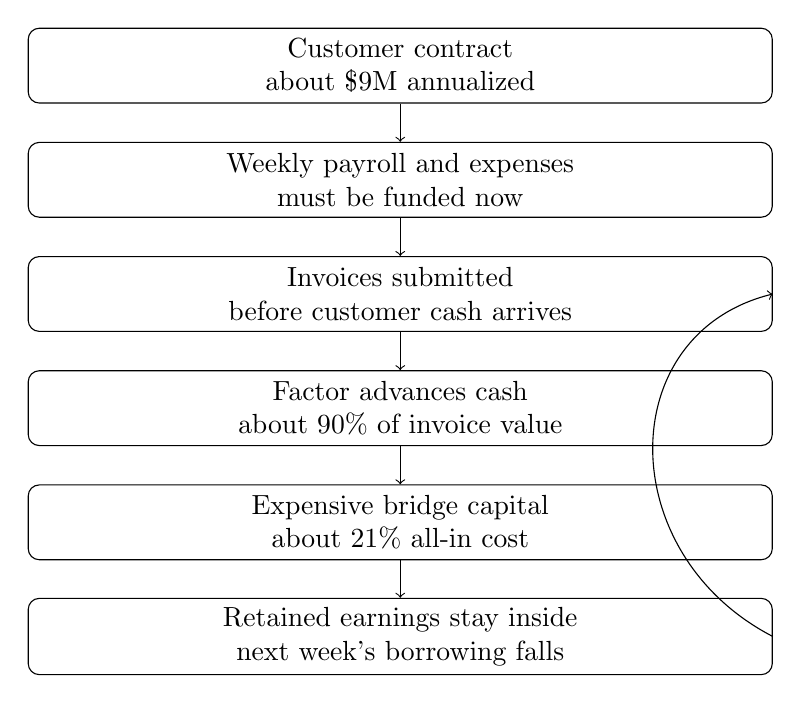
\begin{tikzpicture}[
  node/.style={draw, rounded corners, align=center, text width=0.76\linewidth, minimum height=0.95cm},
  yscale=1.0
]
\node[node] (contract) at (0,0) {Customer contract\\about \$9M annualized};
\node[node] (expense) at (0,-1.45) {Weekly payroll and expenses\\must be funded now};
\node[node] (invoice) at (0,-2.90) {Invoices submitted\\before customer cash arrives};
\node[node] (factor) at (0,-4.35) {Factor advances cash\\about 90\% of invoice value};
\node[node] (cost) at (0,-5.80) {Expensive bridge capital\\about 21\% all-in cost};
\node[node] (retain) at (0,-7.25) {Retained earnings stay inside\\next week's borrowing falls};

\draw[->] (contract) -- (expense);
\draw[->] (expense) -- (invoice);
\draw[->] (invoice) -- (factor);
\draw[->] (factor) -- (cost);
\draw[->] (cost) -- (retain);
\draw[->] (retain.east) .. controls (2.7,-6.2) and (2.7,-3.4) .. (invoice.east);
\end{tikzpicture}
\caption{Transcript-derived working-capital bridge. The factoring loop is painful, but retained earnings reduce the borrowing need over time.}
\end{figure}

The important narrative reversal is that painful financing became a teacher. Louis calls the factoring money horrible and compares it to loan-shark money. Yet he also says it taught financial discipline. He could not take money out. He had to leave money inside the company so that the next week's borrowing would be a little smaller.

\section{From Ten to One Hundred: Customers and Capital Together}

The interviewer then asks how Louis went from a \$10 million company to a \$100 million company. Louis does not answer with a single trick. He says the company had to focus on customers and, at the same time, fund the growth.

The customer side was consultative:
\begin{itemize}
\item make the customer's business better,
\item make the customer more profitable,
\item make the customer more competitive,
\item earn the right to do more business together.
\end{itemize}

The capital side was retained earnings and a stronger balance sheet. These two sides have to move together. Customers without capital create strain. Capital without customer demand creates idle capacity.

\begin{equation}
\text{scalable growth}
\approx
\text{signed customer demand}
+
\text{capital to fund delivery}.
\end{equation}

\subsection{Question \& Answer}

\paragraph{Question.} What had to happen at the same time?

\paragraph{Answer.} Louis says he needed people who believed in the service and were willing to sign contracts, and he needed the money to fund that growth. Both had to happen. A contract is not just revenue on paper; in this business it creates a funding obligation before it becomes collected cash.

\begin{table}
\centering
\begin{tabular}{p{0.28\linewidth} p{0.30\linewidth} p{0.32\linewidth}}
\hline
Mechanism & Transcript evidence & Business meaning \\
\hline
Delegation & \$300M versus maybe \$3M & One person's labor became organizational capacity \\
Retained earnings & Cash stayed in the company & Borrowing need fell week by week \\
Factoring & 90\% advance, 21\% cost & Expensive bridge from invoice to cash \\
Customer focus & Make client more profitable & Sales tied to measurable customer value \\
SOPs & Repeatable daily procedures & New sites could be operated consistently \\
Authority & Accountability requires authority & Delegation requires decision rights \\
Bank relationships & Nearly \$14M borrowing need & Credibility and balance sheet unlocked cheaper credit \\
\hline
\end{tabular}
\caption{Transcript-grounded mechanisms in Louis's scaling story.}
\end{table}

\section{SOPs, Culture, and Delegated Authority}

Once the company has customers and capital, the next problem is replication. Louis describes the move from a few successful sites to several new ones. How do we get people to perform daily operating procedures consistently and produce reliable results?

The first answer is training and SOPs. The second answer is culture. The third answer is authority.

A thin version of delegation says, ``give people tasks.'' Louis gives a stronger version:
\begin{equation}
\text{real accountability}
\quad\Rightarrow\quad
\text{real authority}.
\end{equation}
If someone is responsible for outcomes but has no authority to act, then accountability becomes punishment rather than management. Louis says people need the freedom to take risks, push the envelope of the business, and think of things the CEO may not think of.

This becomes an operating principle:
\begin{proposition}
In the interview's model of scale, delegation works only when procedures, authority, and culture are coupled. SOPs make work repeatable; authority lets people act; culture keeps talent committed enough to use that authority well.
\end{proposition}

\begin{proof}
The transcript gives the sequence. New contracts create new operating sites. New sites require consistent daily procedures. Procedures require training. But Louis then says the most vital piece is leadership style and company culture: respect, loyalty, reward, room to make mistakes, and authority before accountability. Therefore the delegated company is not merely a chart of tasks; it is a system that turns distributed judgment into repeatable performance.
\end{proof}

He extends the point to executive meetings. If six people are in the room, he describes himself as number six. The others are there because they know things he does not know. Their job is not simply to agree. They must say where he is wrong, why something will not work, and how the same goal might be achieved another way.

That is the organizational version of leverage. One mind becomes six minds. One owner becomes a room that can challenge, correct, and improve the plan.

\section{Relationships, Bank Credit, and Results-Based Negotiation}

After the internal operating story, the interview turns to relationships. The first external relationship Louis emphasizes is with bankers. The earlier invoice factoring was not the end state; it was a bridge toward a traditional line of credit.

He says he started developing banker relationships before the balance sheet was ready. He let bankers guide him: where does the balance sheet need to be for a line of credit of a given size? By roughly the third year, he recalls borrowing needs of almost \$14 million.

\begin{equation}
L_{\mathrm{bank}} \approx \$14\text{M}
\end{equation}
is the spoken scale of the later credit need. The mechanism is not only financial. It is relational. Bankers saw retained earnings, improving discipline, and wise risk rather than reckless risk.

Louis then broadens relationships to peer groups. He wishes he had joined organizations where owners and CEOs were not trying to sell to one another, but were there to collaborate. The value is time compression: an hour with the right group can save many hours of isolated trial and error.

Finally the interview asks about negotiation. The tension is clear: Louis is relationship-centric, but he has negotiated large seven- and eight-figure deals. What happens when a buyer only cares about price?

\subsection{Question \& Answer}

\paragraph{Question.} How do you negotiate when the buyer only cares about price?

\paragraph{Answer.} Louis says not to get trapped in today's margin fight. If the buyer needs the price win today, let them have that win, but move the negotiation toward measurable long-term results. If the provider saves the customer money, improves the bottom line, reduces cost, or helps the customer grow, then the provider can earn margin on the back side.

A compact version is
\begin{equation}
\text{seller upside}
\propto
\text{measured customer savings or growth}.
\end{equation}

\begin{figure}
\centering
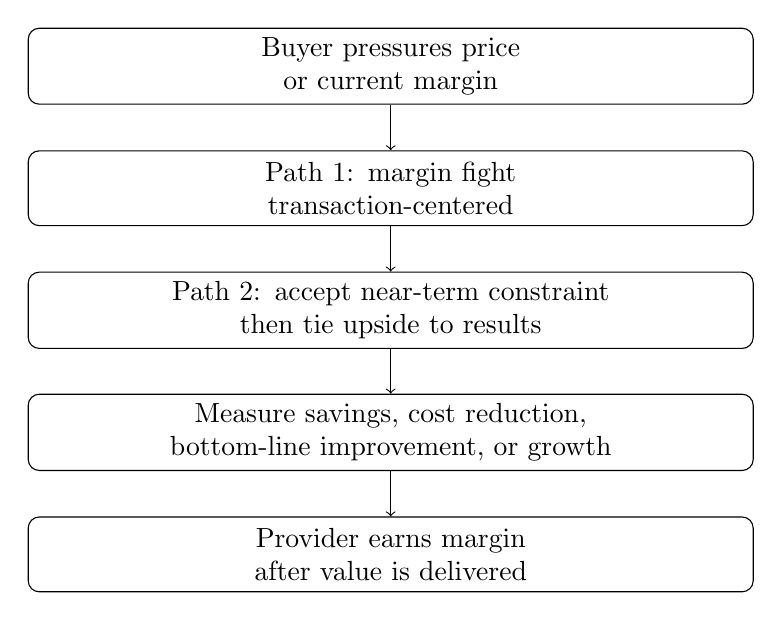
\begin{tikzpicture}[
  node/.style={draw, rounded corners, align=center, text width=0.74\linewidth, minimum height=0.95cm},
  yscale=1.0
]
\node[node] (pressure) at (0,0) {Buyer pressures price\\or current margin};
\node[node] (fight) at (0,-1.55) {Path 1: margin fight\\transaction-centered};
\node[node] (long) at (0,-3.10) {Path 2: accept near-term constraint\\then tie upside to results};
\node[node] (measure) at (0,-4.65) {Measure savings, cost reduction,\\bottom-line improvement, or growth};
\node[node] (payoff) at (0,-6.20) {Provider earns margin\\after value is delivered};

\draw[->] (pressure) -- (fight);
\draw[->] (fight) -- (long);
\draw[->] (long) -- (measure);
\draw[->] (measure) -- (payoff);
\end{tikzpicture}
\caption{Transcript-derived negotiation pattern: escape the price-only fight by tying future compensation to measurable customer results.}
\end{figure}

The negotiation lesson returns us to the earlier customer-focus section. Louis's sales posture was consultative: if he could not make the customer's business better, the customer owed him nothing. The negotiation posture is the same idea in contract form: let the customer pay more only after the provider has made the business better.

\section{Summary}

The interview begins with a Ferrari, but its serious content is not about consumption. It is about the arithmetic of scale. Delegation turns personal labor into organizational capacity. Retained earnings reduce expensive borrowing. Invoice factoring bridges a cash gap but extracts a painful cost. Customer contracts create growth only when the company can fund delivery. SOPs, culture, and authority make delegation repeatable. Bankers, peer groups, and customers become part of the operating system.

The central pattern is simple enough to state as a sequence:
\[
\text{proof}
\rightarrow
\text{cash-flow discipline}
\rightarrow
\text{stronger balance sheet}
\rightarrow
\text{better capital}
\rightarrow
\text{larger contracts}
\rightarrow
\text{delegated scale}.
\]
The transcript's numbers are approximate interview claims, but they carry a clear commercial logic. Wealth arrives here not as a single event, but as a series of constraints survived in the right order.